\documentclass[12pt,a4paper]{article}

\usepackage{graphicx}% Include figure files
\usepackage{dcolumn}% Align table columns on decimal point
\usepackage{bm}% bold math
%\usepackage{hyperref}% add hypertext capabilities
%\usepackage[mathlines]{lineno}% Enable numbering of text and display math
%\linenumbers\relax % Commence numbering lines

%\usepackage[showframe,%Uncomment any one of the following lines to test 
%%scale=0.7, marginratio={1:1, 2:3}, ignoreall,% default settings
%%text={7in,10in},centering,
%%margin=1.5in,
%%total={6.5in,8.75in}, top=1.2in, left=0.9in, includefoot,
%%height=10in,a5paper,hmargin={3cm,0.8in},
%]{geometry}

\usepackage{multicol}%Para hacer varias columnas
\usepackage{multicol,caption}
\usepackage{multirow}
\usepackage{cancel}

\setlength{\topmargin}{-1.0in}
\setlength{\oddsidemargin}{-0.3pc}
\setlength{\evensidemargin}{-0.3pc}
\setlength{\textwidth}{6.75in}
\setlength{\textheight}{9.5in}
\setlength{\parskip}{0.5pc}

\usepackage[utf8]{inputenc}
\usepackage{expl3,xparse,xcoffins,titling,kantlipsum}
\usepackage{graphicx}
\usepackage{xcolor} 
\usepackage{nopageno}
\usepackage{lettrine}
\usepackage{caption}
\captionsetup[table]{name=Tabla}
\renewcommand{\figurename}{Figura}
\usepackage{float}
\renewcommand\refname{Bibliograf\'ia}
\usepackage{amssymb}
\usepackage{amsmath}
\usepackage[rightcaption]{sidecap}
\usepackage[spanish]{babel}

\providecommand{\abs}[1]{\lvert#1\rvert}
\providecommand{\norm}[1]{\lVert#1\rVert}

% CABECERA Y PIE DE PÁGINA %%%%%
\usepackage{fancyhdr}
\pagestyle{fancy}
\fancyhf{}

\begin{document}
Presentación 2
\begin{enumerate}





    \item \textbf{Si $f = f(r)$ con $r = \sqrt{x^2 + y^2 + z^2}$, demuestra que}
    \begin{equation*}
        \nabla f(r) = \hat{r} \frac{df(r)}{dr}
    \end{equation*}
    
    Por la ec. (6), y usando coordenadas esféricas
    
    \begin{equation*}
        \nabla f(r) = \sum_{i=1}^{3} \frac{\hat{e}_i}{h_i} \frac{\partial f(r)}{\partial \theta} = \frac{\hat{e}_r}{h_r} \frac{\partial f(r)}{\partial r} + \frac{\hat{e}_\theta}{h_\theta} \frac{\partial f(r)}{\partial \theta} + \frac{\hat{e}_\phi}{h_\phi} \frac{\partial f(r)}{\partial \phi}
    \end{equation*}
    
    y como f solo depende de r, entonces
    
    \begin{equation*}
        \nabla f(r) = \frac{\hat{e}_r}{h_r} \frac{\partial f (r)}{\partial r}
    \end{equation*}
    
    ahora, como $\textbf{r} = \hat{i} r sen\theta cos\phi + \hat{j} r sen\theta sen \phi + \hat{k}r cos\theta$
    
    \begin{equation*}
        h_r = \norm{\frac{\partial \textbf{r}}{\partial r}} = \sqrt{sen^2\theta cos^2 \phi + sen^2 \theta sen^2 \phi + cos^2 \theta} = \sqrt{sen^2 \theta \cancel{[cos^2\phi +sen^2 \phi]} + cos^2\theta}
    \end{equation*}
    
    \begin{equation*}
        = \sqrt{sen^2\theta + cos^2\theta} = 1
    \end{equation*}
    
    así
    
    \begin{equation*}
        \nabla f(r) = \hat{e}_r \frac{\partial f}{\partial r} = \hat{r} \frac{\partial f}{\partial r}
    \end{equation*}
    

    
    
    
    
    
    \item \textbf{Demuestra que el campo eléctrico de una carga puntual}
    
    \begin{equation*}
        E = \frac{q \hat{r}}{4 \pi \epsilon_o r^2}
    \end{equation*}
    
    \textbf{cumple $\nabla \cdot E = 0$, para $r \neq 0$}
    
    Por la ec. (8), y usando coordenadas esféricas
    \begin{equation*}
        Div E = \frac{1}{h} \sum_{i=1}^{3} \frac{\partial}{\partial u_i}\left(\frac{E_ih}{h_i}\right) = \frac{1}{h}\left[\frac{\partial}{\partial u_r}\left(\frac{E_rh}{h_r}\right) + \frac{\partial}{\partial u_\theta}\left(\frac{E_\theta h}{h_\theta}\right) + \frac{\partial}{\partial u_\phi}\left(\frac{E_\phi h}{h_\phi}\right) \right]
    \end{equation*}
    
    y como E solo tiene componente $E_r$
    \begin{equation*}
        \nabla \cdot E = \frac{1}{h} \frac{\partial}{\partial r} \left( \frac{E_r h}{h_r}\right)
    \end{equation*}
    
    y como ya tenemos $h_r$, solo fatan $h_\theta$ y $h_\phi$
    \begin{equation*}
        h_\theta = \norm{\frac{\partial \textbf{r}}{\partial \theta}} =\sqrt{r^2 cos^2 \theta cos^2 \phi + r^2 cos^2 \theta sen^2 \phi + r^2 sen^2 \theta} = \sqrt{r^2 \left[ cos^2 \theta cos^2 \phi + cos^2\theta sen^2 \phi + sen^2 \theta \right]}
    \end{equation*}
    
    \begin{equation*}
        = r \sqrt{cos^2 \theta \cancel{(cos^2 \phi + \sen^2 \phi)} + sen^2 \theta} = r\sqrt{\cancel{cos^2 \theta + sen^2 \theta}} = r
    \end{equation*}
    
    \begin{equation*}
        h_\phi = \norm {\frac{\partial \textbf{r}}{\partial \theta}} = \sqrt{r^2 sen^2 \theta sen^2 \phi + r^2 sen^2 \theta cos^2 \phi} = \sqrt{r^2\left[sen^2 \theta sen^2 \phi + sen^2 \theta cos^2 \phi  \right]}
    \end{equation*}
    
    \begin{equation*}
        = r \sqrt{sen^2 \theta (\cancel{cos^2 \phi + sen^2 \phi}) } = r sen \theta
    \end{equation*}
    
    así
    
    \begin{equation*}
        \nabla \cdot E = \frac{1}{h_r h_\theta h_\phi} \frac{\partial}{\partial r} \left( \frac{q \cancel{ h_r} h_\theta h_\phi}{4 \pi \epsilon_o r^2 \cancel{h_r}} \right) = \frac{\cancel{sen \theta}}{r^2 \cancel{sen \theta}} \cancel{\frac{\partial}{\partial r} \left(\frac{q \cancel{r^2}}{4\pi \epsilon _o \cancel{r^2}} \right)} =0
    \end{equation*}
    
    para $r\neq0$ (así no se indetermina)
    
    
    
    \item \textbf{La ley de Gauss para el campo eléctrico tiene la forma :}
    
    \begin{equation*}
        \oint E \cdot dS = \frac{q}{\epsilon_o}
    \end{equation*}
    
    \textbf{donde $q = \int \rho dV$ es la carga encerada en la superficie y $\rho$ su densidad volumétrica. Demuestra la ley de Gauss en su forma diferencial}
    
    \begin{equation*}
        \nabla \cdot E = \frac{\rho}{\epsilon_o}
    \end{equation*}
    
    Por el teorema de la divergencia,
    
    \begin{equation*}
        \oint E \cdot dS = \int \nabla \cdot E dV = \frac{q}{\epsilon_o} = \frac{1}{\epsilon_o} \int \rho dV
    \end{equation*}
    
    como la expresión anterior debe ser cierta para cualquier volumen(incluso uno infinitesimal) se tiene que se pueden igualar los integrandos
    
    \begin{equation*}
        \nabla \cdot E = \frac{\rho}{\epsilon_o}
    \end{equation*}
    
    
    
    
    
    \item \textbf{Demuestra que : $\nabla \times (\phi A) = \phi \nabla \times A + \nabla \phi  \times A$}
    
    Usando la ec. (10) en su forma matricial:
    
    \begin{equation*}
    \nabla \times (\phi \textbf{A}) =  \frac{1}{h}
        \begin{vmatrix}
        h_1 \hat{e}_1 & h_2 \hat{e}_2 & h_3 \hat{e}_3\\
        \frac{\partial}{\partial u_1} & \frac{\partial }{\partial u_2} & \frac{\partial}{\partial u_3}\\
        \phi A_1 h_1 & \phi A_2 h_2 & \phi A_3 h_3
        \end{vmatrix}
    \end{equation*}
    
    \begin{equation*}
        = \frac{1}{h} [h_1 \left(\frac{\partial}{\partial u_2}( \phi A_3 h_3) - \frac{\partial }{\partial u_3} (\phi A_2 h_2) \right) \hat{e}_1 - h_2 \left(\frac{\partial}{\partial u_1}( \phi A_3 h_3) - \frac{\partial }{\partial u_3} (\phi A_1 h_1) \right) \hat{e}_2 
    \end{equation*}
    
    \begin{equation*}
         + h_3 \left(\frac{\partial}{\partial u_1}( \phi A_2 h_2) - \frac{\partial }{\partial u_2} (\phi A_1 h_1) \right) \hat{e}_3 ]
    \end{equation*}
    
    o más compacto, usando notación de índices:
    
    \begin{equation*}
        \nabla \times (\phi \textbf{A})_i = \frac{h_i}{h} \epsilon_{ijk} \frac{\partial}{\partial u_j}(\phi A_k h_k) 
    \end{equation*}
    
    ahora metamos el diferencial al paréntesis y reordenemos
    
    \begin{equation*}
        \nabla \times (\phi \textbf{A})_i =\frac{h_i}{h} \epsilon_{ijk} \left[\frac{\partial }{\partial u_j} (\phi) A_k h_k + \phi \frac{\partial}{\partial u_j} (A_k h_k) \right]
    \end{equation*}
    
    cambiemos a la notación presentada en el material adicional de índices
    
    \begin{equation*}
        = \frac{h_i}{h} \epsilon_{ijk} \left[\phi \partial_j (A_k h_k) + \partial_j (\phi) A_k h_k \right]
    \end{equation*}
    
    \begin{equation*}
        \frac{h_i}{h} \phi \epsilon_{ijk} \partial_j (A_k h_k) + \frac{h_i}{h} \epsilon_{ijk} \partial_j(\phi) A_k h_K
    \end{equation*}
    
    \begin{equation*}
        = \phi (\frac{h_i}{h} \epsilon_{ijk} \partial_j A_k h_k) +  (\frac{h_i}{h} \epsilon_{ijk} \partial_j (\phi) A_k h_k)
    \end{equation*}
    
    \begin{equation*}
        = \phi (\nabla \times \textbf{A})_i + (\nabla \phi \times \textbf{A})_i
    \end{equation*}
    
    \begin{equation*}
        \therefore \nabla \times (\phi \textbf{A}) = \phi \nabla \times \textbf{A} + \nabla \phi \times \textbf{A}
    \end{equation*}

    
    
    
    
    
    \item \textbf{El campo electroestático de un dipolo eléctrico $p = p_o \hat{e}_z$ es}
    
    \begin{equation*}
        E = \frac{p_o (2 \hat{e}_r cos \theta + \hat{e}_\theta sen \theta)}{r^3}
    \end{equation*}
    
    \textbf{Demuestra que:}
    \begin{enumerate}
        \item $\nabla \times E = 0$
        
        \item para $r \neq 0$, se tiene $\nabla \cdot E = 0$
    \end{enumerate}
    
    Suponiendo que E está en esféricas, entonces:(y usando los factores de escala calculados en los problemas 1 y 2)
    
    \begin{equation*}
        \nabla \times E = \frac{1}{h}
         \begin{vmatrix}
             h_1 \hat{e}_r & h_2 \hat{e}_\theta & h_3 \hat{e}_\phi\\
             \frac{\partial}{\partial u_r} & \frac{\partial }{\partial u_\theta} & \frac{\partial}{\partial u_\phi}\\
            E_r h_r & E_\theta h_\theta & E_\phi h_\phi
        \end{vmatrix}
    \end{equation*}
    
    \begin{equation*}
    =\frac{1}{r^2 sen\theta} [ \left(\frac{\partial}{\partial \theta} \cancel{(E_\phi r sen \theta)}- \frac{\partial}{\partial \phi} (E_\theta r) \right) \hat{e}_r + r\left( \frac{\partial}{\partial \phi} (E_r) -\frac{\partial}{\partial r}\cancel{(E_\phi r sen \theta)}\right) \hat{e}_\theta +
    \end{equation*}
    
    \begin{equation*}
         r sen \theta \left(\frac{\partial}{\partial r}(E_\theta r) - \frac{\partial}{\partial \theta} (E_r) \right) \hat{e}_\phi]
    \end{equation*}
    
    \begin{equation*}
        = \frac{1}{r\cancel{^2}\cancel{sen \theta}}\left[- \cancel{\frac{\partial}{\partial \phi} (\frac{\rho _0 sen \theta r}{r^3})} \hat{e}_r + r \cancel{\frac{\partial}{\partial \phi}(\frac{2 \rho _0 cos \theta}{r^3})} \hat{e}_\theta + \cancel{r sen \theta}(\frac{\partial}{\partial r}(\frac{\rho _0 sen \theta r}{r^2}) - \frac{\partial}{\partial \theta}(\frac{2 \rho _0 cos \theta}{r^3})) \hat{e}_\phi \right]
    \end{equation*}
    
    \begin{equation*}
        = \frac{1}{r} \left((0) \hat{e}_r + (0) \hat{e}_\theta + \cancel{(\frac{-2 \rho _0 sen \theta}{r^3} - (- \frac{2 \rho _0 sen \theta}{r^3}))} \hat{e}_\phi\right)
    \end{equation*}
    
    \begin{equation*}
        = (0, 0, 0)  \forall r \neq 0
    \end{equation*}
    
    \begin{equation*}
        \nabla \cdot E = \frac{1}{h} \left[\frac{\partial}{\partial r}(\frac{E_r h}{h_r}) + \frac{\partial}{\partial \theta}(\frac{E_\theta h}{h_\theta}) + \frac{\partial}{\partial \phi}(\frac{E_\phi h}{h_\phi}) \right]
    \end{equation*}
    
    \begin{equation*}
        = \frac{1}{r^2 sen \theta} \left[\frac{\partial}{\partial r}(E_r r^2 sen \theta) + \frac{\partial}{\partial \theta}(\frac{E_\theta r \cancel{^2}sen \theta}{\cancel{r}}) + \frac{\partial }{\partial \phi} (\frac{\cancel{E_\phi} r \cancel{^2} \cancel{sen \theta}}{\cancel{r sen \theta}})  \right]
    \end{equation*}
    
    \begin{equation*}
        = \frac{1}{r^2 sen \theta} \left[\frac{\partial}{\partial r}(\frac{2\rho _0 cos \theta \cancel{r^2}sen \theta}{r \cancel{^3}}) + \frac{\partial}{\partial \theta} (\frac{\rho _0 sen^2 \theta \cancel{r}}{r \cancel{^3}}) \right]
    \end{equation*}
    
    \begin{equation*}
        = \frac{1}{r^2 sen \theta} \left[\frac{-2\rho _0cos \theta sen \theta}{r^2} + \frac{2 \rho _0 sen \theta cos \theta}{r^2} \right] = \frac{1}{r^2 sen \theta} [0] = 0
    \end{equation*}
    
    \item \textbf{Demuestra que el Laplaciano en coordenadas cilíndricas y esféricas es el
    que se presenta, para ello tendrás que calcular los respectivos factores
    de escala.}
    
    de la ecuación (12) se sigue que:
    
    \begin{equation*}
        \nabla ^2 f = \frac{1}{h} \sum_{i=1}^{3} \frac{\partial}{\partial u_i}(\frac{h}{h_i^2} \frac{\partial f}{\partial u_i})
    \end{equation*}
    
    con coordenadas esféricas, del ejercicio 1 y 2 se tiene:
    
    \begin{equation*}
        h_r = 1 ; h_\theta = r ; h_\psi = r \sen{\theta}
    \end{equation*}
    
    \begin{equation*}
        \therefore \nabla ^2 f = \frac{1}{r^2 \sen{\theta}} \left[\frac{\partial}{\partial r}(r^2 \sen{\theta}\frac{\partial f}{\partial r}) + \frac{\partial}{\partial \theta}(\frac{\cancel{r^2}\sen{\theta}}{\cancel{r^2}}\frac{\partial f}{\partial \theta}) + \frac{\partial}{\partial \psi}( \frac{\cancel{r^2 \sen{\theta}}}{\cancel{r^2}\cancel{\sen{\theta}}^2} \frac{\partial f}{\partial \psi}) \right]
    \end{equation*}
    
    \begin{equation*}
        = \frac{1}{r^2 \sen{\theta}} \left[\sen{\theta} \frac{\partial}{\partial r}(r^2 \frac{\partial f}{\partial r}) + \frac{\partial}{\partial \theta}(\sen{\theta}\frac{\partial f}{\partial \theta}) +  \frac{1}{\sen{\theta}}\frac{\partial^2 f}{\partial \psi ^2} \right]
    \end{equation*}
    
    \begin{equation*}
        = \frac{1}{r^2} \frac{\partial}{\partial r}(r^2 \frac{\partial f}{\partial r}) + \frac{1}{r^2 \sen{\theta}} \frac{\partial}{\partial \theta}(\sen{\theta} \frac{\partial f}{\partial \theta}) + \frac{1}{r^2 \sen{\theta}} \frac{\partial ^2 f}{\partial \psi ^2}
    \end{equation*}
    
    en coordenadas cilíndricas, dado que:
    
    \begin{equation*}
        \textbf{r} = \hat{\imath} \rho \cos{\psi} + \hat{\jmath} \rho \sen{\psi} + \hat{k} z
    \end{equation*}
    
    entonces:
    
    \begin{equation*}
        \frac{\partial \textbf{r}}{\partial \rho} = \hat{\imath} \cos{\psi} + \hat{\jmath} \sen{\psi}
    \end{equation*}
    
    \begin{equation*}
        \frac{\partial \textbf{r}}{\partial \psi} = - \hat{\imath} \rho \sen{\psi} + \hat{\jmath} \rho \cos{\psi}
    \end{equation*}
    
    \begin{equation*}
        \frac{\partial \textbf{r}}{\partial z} = \hat{k}
    \end{equation*}
    
    así:
    
    \begin{equation*}
        h_\rho = \norm{\frac{\partial \textbf{r}}{\partial \rho}} = \sqrt{\cos^2{\psi} + \sen^2{\psi}} = 1
    \end{equation*}
    
    \begin{equation*}
        h_\psi = \norm{\frac{\partial \textbf{r}}{\partial \psi}} = \sqrt{\rho ^2 \sen^2{\psi} + \rho ^2 \cos^2{\psi}} = \rho \sqrt{\sen^2{\psi} + \cos^2{\psi}} = \rho
    \end{equation*}
    
    \begin{equation*}
        h_z = \norm{\frac{\partial \textbf{r}}{\partial z}} = \sqrt{1} = 1
    \end{equation*}
    
    \begin{equation*}
        \therefore \nabla ^2 f = \frac{1}{\rho} \left[\frac{\partial}{\partial \rho} (\rho \frac{\partial f}{\partial \rho}) + \frac{\partial}{\partial \psi} ( \frac{\cancel{\rho}}{\rho^\cancel{2}} \frac{\partial f}{\partial \psi}) + \frac{\partial}{\partial z} ( \rho \frac{\partial f}{\partial z}) \right]
    \end{equation*}
    
    \begin{equation*}
        = \frac{1}{\rho} \left[\frac{\partial}{\partial \rho} (\rho \frac{\partial f}{\partial \rho}) + \frac{1}{\rho} \frac{\partial^2 f}{\partial \psi^2} + \rho \frac{\partial ^2 f}{\partial z^2} \right]
    \end{equation*}
    
    \begin{equation*}
        = \frac{1}{q} \frac{\partial}{\partial \rho} (\rho \frac{\partial f}{\partial \rho}) + \frac{1}{\rho^2} \frac{\partial^2 f}{\partial \psi ^2}+ \frac{\partial^2 f}{\partial z^2}
    \end{equation*}
    
\end{enumerate}

Presentación 3

\begin{enumerate}
    \item \textbf{Para el sistema de coordenadas esferoidales prolatas $(\xi, \eta, \phi)$, cuyas reglas de transformación son:}
    
    \begin{equation*}
        x = a \senh{\xi} \sen{\eta} \cos{\phi} 
    \end{equation*}
    \begin{equation*}
        y = a \senh{\xi} \sen{\eta} \sen{\phi}
    \end{equation*}
    \begin{equation*}
        z = a \cosh{\xi} \cos{\eta} 
    \end{equation*}
    
    \begin{enumerate}
        \item \textbf{Describe las superficies coordenadas del sistema}
        
        Siguiendo el procedimiento de las notas, elevemos al cuadrado x, y, z:
        
        \begin{equation*}
            x^2 = a^2 \senh^2{\xi} \sen^2{\eta} \cos^2{\phi}
        \end{equation*}
        
        \begin{equation*}
            y^2 = a^2 \senh^2{\xi} \sen^2{\eta} \sen^2{\phi}
        \end{equation*}
        
        \begin{equation*}
            z^2 = a^2 \cosh^2{\xi} \cos^2{\eta}
        \end{equation*}
        
        Ahora desarrollando:
        
        \begin{equation*}
            \frac{x^2 + y^2}{a^2 \senh^2{\xi}} + \frac{z^2}{a^2 \cosh^2{\xi}} = \frac{\cancel{a^2 \senh^2{\xi}} \sen^2{\eta}(\cancel{\cos^2{\phi + \sen^2{\phi}})}}{\cancel{a^2 \senh^2{\xi}}} + \frac{\cancel{a^2 \cosh^2{\xi}}\cos^2{\eta}}{\cancel{a^2 \cosh^2{\eta}}}
        \end{equation*}
        
        \begin{equation*}
            = \cancel{\sen^2{\eta} + \cos^2{\eta}} = 1
        \end{equation*}
        
        \begin{equation*}
            \frac{x^2 + y^2}{a^2 \senh^2{\eta}} - \frac{z^2}{a^2 \cosh^2{\eta}} = \frac{\cancel{a^2 \sen^2{\eta}} \senh^2{\xi} (\cancel{\cos^2{\phi} + \sen^2{\phi}})}{\cancel{a^2 \sen^2{\eta}}} - \frac{\cancel{a^2 \cos^2{\eta}} \cosh^2{\xi}}{\cancel{a^2 \cos^2{\eta}}}
        \end{equation*}
        
        \begin{equation*}
            = \senh^2{\xi} - \cosh^2{\xi} = -(\cancel{\cosh^2{\xi} - \senh^2{\xi}}) = 1
        \end{equation*}
        
        y así,
        
        \begin{equation}
            \frac{x^2 + y^2}{a^2 \senh^2{\xi}} + \frac{z^2}{a^2 \cosh^2{\xi}} = 1
        \end{equation}
        
        \begin{equation}
            \frac{z^2}{a^2 \cos^2{\eta}} - \frac{x^2 + y^2}{a^2 \sen^2{\eta}} = 1
        \end{equation}
        
        Si $\xi = cte$, la ec. (1) tiene la forma de una elipsoide degenerada (esferoide) ($\frac{x^2}{a^2} + \frac{y^2}{a^2} + \frac{z^2}{b^2} = 1$) con ejes, $a \senh{\xi}$ y $a \cosh{\xi}$
        
        Si $\eta = cte$, la ec. (2) tiene la forma de un hiperboloide(hiperboloide de revolución) ($- \frac{x^2}{a^2} - \frac{y^2}{b^2} + \frac{z^2}{c^2} = 1$)
        
        Si
        
        \begin{equation*}
            \phi = cte   \Rightarrow r^2 = x^2 + y^2 + (z\pm a)^2 = x^2 + y^2 +z^2 \pm 2az + a^2
        \end{equation*}
        
        \begin{equation*}
            = a^2 \senh^2{\xi} \sen^2{\eta} \cos^2{\phi} +a^2 \senh^2{\xi} \sen^2{\eta} \sen^2{\phi}+ a^2 \cosh^2{\xi} \cos^2{\eta} \pm 2a^2 \cos{\xi} \cos{\eta} + a^2 
        \end{equation*}
        
        \begin{equation*}
            =a^2 [\senh^2{\xi} \sen^2{\eta}(\cancel{\sen^2{\phi}+\cos^2{\phi}})+ \cosh^2{\xi} \cos^2{\eta} \pm 2\cos{\xi} \cos{\eta}+1]
        \end{equation*}
        
        \begin{equation*}
            =a^2 [(\cosh^2{\xi}-1)\sen^2{\eta}+ \cosh^2{\xi} \cos^2{\eta} \pm 2\cos{\xi}\cos{\eta}+1]
        \end{equation*}
        
        \begin{equation*}
            =a^2[cosh^2{\xi}(\cancel{\sen^2{\eta} + cos^2{\eta}}) - \sen^2{\eta} \pm 2 \cos{\xi} \cos{\eta} + 1]
        \end{equation*}
        
        \begin{equation*}
            = a^2 [\cosh^2{\xi} + \cos^2{\eta}-\cancel{1} \pm 2 \cos{\xi} \cos{\eta} + \cancel{1}]
        \end{equation*}
        
        \begin{equation*}
            = a^2 (\cos{\xi} \pm \cos{\eta})^2
        \end{equation*}
        
        Lo que describe un plano (o la mitad de uno)
        
        \begin{figure}[h!]
            \centering
            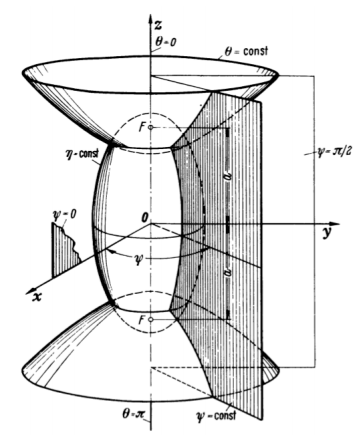
\includegraphics[scale = 1.1]{1.PNG}
        \end{figure}
        
        \item \textbf{Calcula de manera explícita los factores de escala $(h_\xi, h_\eta, h_\phi)$}
        
        Como $\textbf{r} = a \senh{\xi} \sen{\eta} \cos{\phi} \hat{\imath} + a \senh{\xi} \sen{\eta} \sen{\phi} \hat{\jmath} + a \cosh{\xi} \cos{\eta} \hat{k}$
        
        así,
        
        \begin{equation*}
            h_\xi = \norm{\frac{\partial \textbf{r}}{\partial \xi}} = \sqrt{a^2 \sen^2{\eta} \cos^2{\phi}\cosh^2{\phi}+ a^2 \sen^2{\eta}+\sen^2{\phi} \cosh^2{\xi} + a^2 \cos^2{\eta} \senh^2{\xi}}
        \end{equation*}
        
        \begin{equation*}
            = a\sqrt{\sen^2{\eta} \cosh^2{\xi}(\cancel{\cos^2{\phi} + \sen^2{\phi}}) + \cos^2{\eta} \senh^2{\xi}}
        \end{equation*}
        
        \begin{equation*}
            = a \sqrt{\sen^2{\eta}(\senh^2{\xi}+1) + \cos^2{\eta} \senh^2{\xi}}
        \end{equation*}
        
        \begin{equation*}
            = a \sqrt{\senh^2{\xi}(\sen^2{\eta} + \cos^2{\eta}) + \sen^2{\eta}}= a\sqrt{\senh^2{\xi} + \sen^2{\eta}}
        \end{equation*}
        
        \begin{equation*}
            h_\eta = \norm{\frac{\partial \textbf{r}}{\partial \eta}} =\sqrt{a^2 \senh^2{\xi}\cos^2{\eta}\cos^2{\phi} + a^2 \senh^2{\xi}\cos^2{\eta}\sen^2{\phi} + a^2 \cosh^2{\xi}\sen^2{\eta}}
        \end{equation*}
        
        \begin{equation*}
           =a\sqrt{\senh^2{\xi}\cos^2{\eta}(\cancel{\cos^2{phi} + \sen^2{\phi}}) + \cosh^2{\xi} \sen^2{\eta}}
        \end{equation*}
        
        \begin{equation*}
            = a \sqrt{\senh^2{\xi} (1 - \sen^2{\eta}) + \cosh^2{\xi} \sen^2{\eta}}
        \end{equation*}
        
        \begin{equation*}
            = a\sqrt{\senh^2{\xi}+\sen^2{\eta} (\cancel{\cosh^2{\xi} - \senh^2{\xi}})} = h_\xi
        \end{equation*}
        
        \begin{equation*}
            h_\phi = \norm{\frac{\partial \textbf{r}}{\partial \phi}} = \sqrt{a^2\senh^2{\xi}\sen^2{\eta}\sen^2{\phi} + a^2 \sen^2{\xi} \sen^2{\eta}\cos^2{\phi}}
        \end{equation*}
        
        \begin{equation*}
            = a \sqrt{\senh^2{\xi}\sen^2{\eta}(\cancel{\sen^2{\phi} + \cos^2{\phi}})} = a \senh{\xi}\sen{\eta}
        \end{equation*}
        
    \end{enumerate}
    
    \item \textbf{Ocupando el mismo sistema de coordenadas esferoidales prolatas $(\xi, \eta, \psi)$ del ejercicio anterior:}
    
    \begin{enumerate}
        \item \textbf{Calcula los operadores diferenciables $\nabla \phi$, $\nabla \cdot B$, $\nabla \times B$ y $\nabla ^2 \phi$}
        
        Usaremos los facores de escala calculados anteriormente:
        
        \begin{equation*}
            \nabla \phi = \sum \frac{\hat{e_i}}{h_i} \frac{\partial \phi}{\partial u_i} = \frac{\hat{e_\xi}}{h_\xi} \frac{\partial \phi}{\partial \xi} + \frac{\hat{e_\eta}}{h_\eta} \frac{\partial \phi}{\partial \eta} + \frac{\hat{e_\psi}}{h_\psi} \frac{\partial \phi}{\partial \psi}
        \end{equation*}
            
        \begin{equation*}
            = \frac{\hat{e_\xi}}{a \sqrt{\senh^2{\xi}+\sen^2{\eta}}} \frac{\partial \phi}{\partial \xi} + \frac{\hat{e_\eta}}{a \sqrt{\senh^2{\xi} + \sen^2{\eta}}} \frac{\partial \phi}{\partial \eta} + \frac{\hat{e_\psi}}{a \senh{\xi} \sen{\eta}} \frac{\partial \phi}{\partial \psi}
        \end{equation*}
        
        \begin{equation*}
            = \frac{1}{a}\left[\frac{1}{\sqrt{\senh^2{\xi} + \sen^2{\eta}}} (\hat{e_\xi} \frac{\partial \phi}{\partial \xi} + \hat{e_\eta}\frac{\partial \phi}{\partial \eta})+ \frac{\hat{e_\psi}}{\senh{\xi} \sen{\eta}} \frac{\partial \phi}{\partial \psi} \right]
        \end{equation*}
        
        \vspace{1.7cm}
        
        \begin{equation*}
            \nabla \cdot B = \frac{1}{h} \sum \frac{\partial}{\partial u_i} \left(\frac{B_i h}{h_i} \right)= \frac{1}{h} \left[\frac{\partial}{\partial \xi}(\frac{B_\xi \cancel{h}}{\cancel{h_\xi}}) + \frac{\partial}{\partial \eta} (\frac{B_\eta\cancel{h}}{\cancel{h_\eta}}) + \frac{\partial}{\partial \psi} (\frac{B_\psi \cancel{h}}{\cancel{h_\psi}} \right]
        \end{equation*}
        
        \begin{equation*}
            = \frac{1}{h_\xi h_\eta h_\psi} \left[\frac{\partial}{\partial \xi}(B_\xi h_\eta h_\psi) + \frac{\partial}{\partial \eta} (B_\eta h_\xi h_\psi) + \frac{\partial}{\partial \psi}(B_\psi h_\xi h_\psi) \right]
        \end{equation*}
        
        \begin{equation*}
            = \frac{\cancel{a^2}}{a\cancel{^3} (\senh^2{\xi} + \sen^2{\eta})\senh{\xi} \sen{\eta}}[ \frac{\partial}{\partial \xi} (B_\xi \sqrt{\senh^2{\xi} +\sen^2{\eta}} \senh{\xi} \sen{\eta}) +
        \end{equation*}
        
        \begin{equation*}
             \frac{\partial}{\partial \eta} (B_\eta \sqrt{\senh^2{\xi} + \sen^2{\eta}}\senh{\xi}) +\frac{\partial}{\partial \psi} (B_\psi (\sen^2{\xi} + \sen^2{\xi})]
        \end{equation*}
        
        \vspace{1.7cm}
        
        \begin{equation*}
            \nabla \times B =  = \frac{1}{h}
            \begin{vmatrix}
                h_\xi \hat{e}_\xi & h_\eta \hat{e}_\eta & h_\psi \hat{e}_\psi\\
                \frac{\partial}{\partial \xi} & \frac{\partial }{\partial \eta} & \frac{\partial}{\partial u_\psi}\\
                B_\xi h_\xi & B_\eta h_\eta & B_\psi h_\psi
            \end{vmatrix}
        \end{equation*}
        
        \begin{equation*}
            =\frac{1}{h}[h_\xi(\frac{\partial}{\partial \eta}(B_\psi h_\psi) - \frac{\partial}{\partial \psi}(B_\eta h_\eta)) \hat{e}_\xi + h_\eta(\frac{\partial}{\partial \psi}(B_\xi h_\xi) - \frac{\partial}{\partial \xi}(B_\psi h_\psi))\hat{e}_\eta +
        \end{equation*}
        
        \begin{equation*}
             h_\psi (\frac{\partial}{\partial \xi}(B_\eta h_\eta) - \frac{\partial}{\partial \eta}(B_\xi h_\xi))\hat{e}_\psi]
        \end{equation*}
        
        \begin{equation*}
            = \frac{1}{h_\xi h_\psi}(\frac{\partial}{\partial \eta} (B_\psi h_\psi)- \frac{\partial}{\partial \psi} (B_\eta h_\eta)) \hat{e}_\xi + \frac{1}{h_\xi h_\psi} (\frac{\partial}{\partial \psi}(B_\xi h_\xi) - \frac{\partial}{\partial \xi}(B_\psi h_\psi)) \hat{e}_\xi +
        \end{equation*}
        
        \begin{equation*}
            \frac{1}{h_\xi h_\eta}(\frac{\partial}{\partial \xi}(B_\eta h_\eta)- \frac{\partial}{ \partial \eta}(B_\xi h_\xi)) \hat{e}_\psi
        \end{equation*}
        
        \begin{equation*}
            = \frac{1}{a\cancel{^2} \senh{\xi}\sen{\eta}\sqrt{\senh^2{\xi} + \sen^2{\eta}}}(\frac{\partial}{\partial \eta}(B_\psi \cancel{a}\senh{\xi} \sen{\eta}) - \frac{\partial}{\partial \psi}(B_\eta  \cancel{a} \sqrt{\senh^2{\xi}+ \sen^2{\eta}}) \hat{e}_\xi
        \end{equation*}
        
        \begin{equation*}
            + \frac{1}{a\cancel{^2}\senh{\xi}\cancel{\sen{\eta}} \sqrt{\senh^2{\xi}+ \sen^2{\eta}}} (\frac{\partial}{\partial \psi} (B_\xi \cancel{a \sen{\eta}}\sen{\xi}) - \frac{\partial}{\partial \xi}(B_\psi \cancel{a \sen{\eta}} \senh{\xi})) \hat{e}_\eta
        \end{equation*}
        
        \begin{equation*}
            + \frac{1}{a\cancel{^2} (\senh^2{\xi} + \sen^2{\eta})}(\frac{\partial}{\partial \xi}(B_\eta \cancel{a} \sqrt{\senh^2{\xi} + \sen^2{\eta}}) - \frac{\partial}{\partial \eta}(B_\xi \cancel{a} \sqrt{\senh^2{\xi} + \en^2{\eta}})) \hat{e}_\psi
        \end{equation*}
        
        \begin{equation*}
            = \frac{1}{a \sqrt{\senh^2{\xi} + \sen^2{\eta}}}(\frac{\frac{\partial}{\partial \eta}(B_\eta \sen{\eta})}{\sen{\eta}} - \frac{\sqrt{\senh^2{\xi} + \sen^2{\eta}} \frac{\partial}{\partial \xi} B_\eta}{\senh{\xi} \sen{\eta}} + \frac{\partial}{\partial \psi} B_\xi - \frac{\frac{\partial}{\partial \xi}(B_\psi \senh{\xi})}{\senh{\xi}}
        \end{equation*}
        
        \begin{equation*}
            + \frac{\frac{\partial}{\partial \xi}(B_\eta \sqrt{\senh^2{\xi} + \sen^2{\eta}})}{\sqrt{\senh^2{\xi} + \sen^2{\eta}}} - \frac{\frac{\partial}{\partial \eta}(B_\xi \sqrt{\sen^2{\xi} + \sen^2{\eta}})}{\sqrt{\senh^2{\xi} + \sen^2{\eta}}})
        \end{equation*}
        
        
        
        
        
        
        
        \newpage
        
        
        \begin{equation*}
            \nabla^2 \phi = \frac{1}{h} \sum \frac{\partial}{\partial u_i}\left(\frac{h}{h_i ^2}\frac{\partial \phi}{\partial u_i} \right)
        \end{equation*}
        
        \begin{equation*}
            = \frac{1}{h}\left[\frac{\partial}{\partial \xi}(\frac{h}{h_\xi ^2}\frac{\partial \phi}{\partial \xi}) + \frac{\partial}{\partial \eta} (\frac{h}{h_\eta ^2} \frac{\partial \phi}{\partial \eta}) + \frac{\partial}{\partial \psi}(\frac{h}{h_\psi ^2} \frac{\partial \phi}{\partial \psi}) \right]
        \end{equation*}
        
        \begin{equation*}
            = \frac{1}{h} \left[\frac{\partial}{\partial \xi} (h_\psi \frac{\partial \phi}{\partial \xi}) + \frac{\partial}{\partial \eta}(h_\psi \frac{\partial \phi}{\partial \eta}) + \frac{\partial}{\partial \psi}(\frac{a(\senh^2{\xi} + \sen^2{\eta})}{\senh{\xi}\sen{\eta}}\frac{\partial \phi}{\partial \psi}) \right]
        \end{equation*}
        
        \begin{equation*}
            = \frac{1}{a\cancel{^3} (\senh^2{\xi} + \sen^2{\eta})\senh{\xi}\sen{\eta}}[\frac{\partial}{\partial \xi}(\cancel{a} \senh{\xi}\sen{\eta} \frac{\partial \phi}{\partial \xi}) + \frac{\partial}{\partial \eta} (\cancel{a}\senh{\xi} \sen{\eta} \frac{\partial \phi}{\partial \eta}) +
        \end{equation*}
        
        \begin{equation*}
             \frac{\cancel{a}(\sen^2{\xi} +\sen^2{\eta})}{\senh{\xi} \sen{\eta}} \frac{\partial^2 \phi}{\partial \psi^2}]
        \end{equation*}
        
        \begin{equation*}
            =\frac{1}{a^2 (\senh^2{\xi}+\sen^2{\eta})\senh{\xi}\sen{\eta}}[\sen{\eta}\frac{\partial}{\partial \xi} (\senh{\xi} \frac{\partial \phi}{\partial \xi}) + \senh{\xi}\frac{\partial}{\partial \eta}(\sen{\eta} \frac{\partial \phi}{\partial \eta})+ 
        \end{equation*}
        
        \begin{equation*}
            \frac{\senh^2{\xi}+\sen^2{\eta}}{\senh{\xi}\sen{\eta}} \frac{\partial^2 \phi}{\partial \psi^2}]
        \end{equation*}
        
        
    \end{enumerate}
\end{enumerate}


\end{document}
